% A deep neural network with 3 hidden layers of varying sizes.

\begin{figure}[htbp]
\renewcommand{\familydefault}{\sfdefault}\normalfont
\centering

\def\layersep{1.5cm}

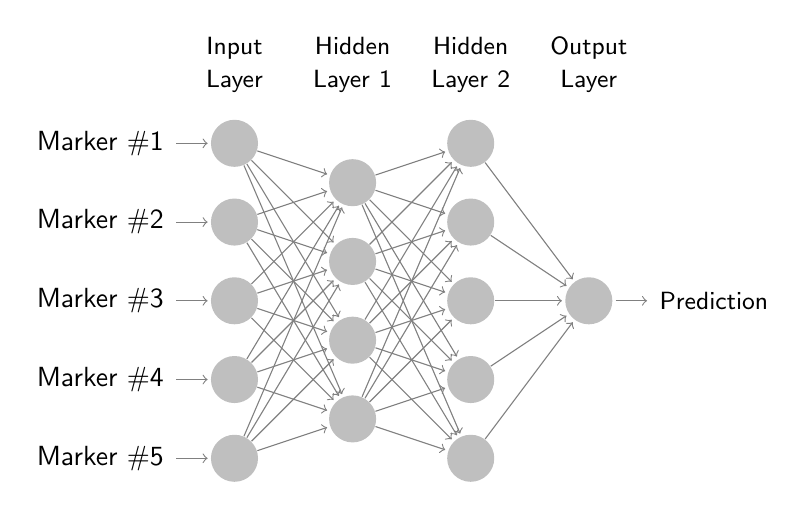
\begin{tikzpicture}[shorten >=1pt, ->, draw=black!50, node distance=\layersep]
    \tikzstyle{every pin edge}=[<-, shorten <=1pt]

    \tikzstyle{neuron}=[circle, fill=black!25,minimum size=17pt, inner sep=0pt]
    \tikzstyle{input neuron}=[neuron];
    \tikzstyle{output neuron}=[neuron];
    \tikzstyle{hidden neuron}=[neuron];

    \tikzstyle{annot}=[text width=4em, text centered]

    \foreach \name / \y in {1,...,5}
        \node[input neuron, pin=left:Marker \#\y] (I-\name) at (0,-\y) {};

    \foreach \name / \y in {1,...,4}
        \path[yshift=-0.5cm]
            node[hidden neuron] (H1-\name) at (\layersep * 1,-\y cm) {};

    \foreach \name / \y in {1,...,5}
        \path[yshift=0.0cm]
            node[hidden neuron] (H2-\name) at (\layersep * 2,-\y cm) {};

    \node[output neuron, pin={[pin edge={->}]right:\small{Prediction}}, right of=H2-3] (out) {};

    \foreach \source in {1,...,5}
        \foreach \dest in {1,...,4}
            \path (I-\source) edge (H1-\dest);

    \foreach \source in {1,...,4}
        \foreach \dest in {1,...,5}
            \path (H1-\source) edge (H2-\dest);

    \foreach \source in {1,...,5}
        \path (H2-\source) edge (out);

    \node[annot, above of=I-1, node distance=1cm] (il) {\small Input Layer};
    \node[annot, right of=il] (hl1) {\small Hidden Layer 1};
    \node[annot, right of=hl1] (hl2) {\small Hidden Layer 2};
    \node[annot, right of=hl2] {\small Output Layer};
\end{tikzpicture}

\caption{A deep feedforward neural network. Many input marker calls are mapped 
         to one or more sequential hidden layers of neurons. For genomic prediction, the 
         input layer often consists of one neuron per marker and the output consists of a single
         neuron which combines the information from the final hidden layer to predict a phenotype or BLUP.
         The presence of more than one hidden layer indicates that a network that may be more likely to learn
         higher order non-linear interactions, and can be called a deep network.}
\label{fig:deepnet}
\end{figure}
